\begin{abstract}
As electronic devices get increasingly personalized,
mixed signal integrated circuits such as analog to digital converters (ADCs)
and digital to analog converters (DACs) play a pivotal role in interfacing 
between the real world and the digital domain. Side-by-side, the security
requirements of these devices are increasing manifold. Many of these devices
require to be authenticated and have built in techniques to support 
encryption and prevent counterfeiting. For embedded devices, 
these requirements are efficiently implemented by 
using physically unclonable functions (or PUFs) that make use of the 
unique nanoscale variations during device fabrication.

In this paper, we show how mixed signal ICs in a device like ADCs and DACs 
have properties that make them amicable for use in PUF applications. By
virtue of having analog components, the PUF properties in these ICs
are significantly more amplified compared to digital PUFs such as those based on
SRAM and ring oscillators. An added advantage is that mixed signal PUFs
have considerably less overheads compared to the contemporary digital PUFs. 
\end{abstract}

\section{Introduction}
The physical characteristics of every electronic device is unique.
The uniqueness is due to micro and nanoscale variations in the 
silicon substrate and fabrication process. A physically unclonable function 
(or PUF) uses this uniqueness to provide a cryptographic key that 
cannot be forged. PUFs have wide application, especially for device
authentication, anti-counterfeiting, and tamper resistance.
Unlike contemporary techniques of storing keys in memory,
PUFs utilize a series of challenges and responses. Each response is a 
function of the challenge and device characteristics. 

Several PUFs have been constructed over the years. Most of them
from electronic components such as the SRAM, ring oscillators, flip flops,
FPGA units etc. A few non-electronic PUFs such as optical, acoustic,
and magnetic PUFs have also been proposed. The important requirements
for a PUF is that they should be compact, unforgeable, unpredictable, irreversible, 
reliable, and easy to evaluate. These requirements are easier said than done.
Many of the requirements are contrasting, while many are drastically affected
by noise and other environmental factors such as the ambient temperature.
Thus the search for the search for the perfect PUF is an open problem
and active area of research.


These requirements should be met 
irrespective of the noise and other environmental factors. 




In this demonstrate, we hope to build a PUF based on analog to digital
converters (ADCs). These devices are widely used in wireless sensor nodes
and also integrated into many low cost micro-controllers.
Compared to other electronic PUFs, ADC PUFs may not require any 
special hardware such as oscillators, arbiters, etc. They would thus
be compact. The plan is to feed analog waveforms to the ADC (challenges) 
under varying conditions and collect the converted digital outputs 
(responses). The responses would then be analyzed for PUF properties 
such as reproducibility, uniqueness, unclonability, unpredictability, 
one-wayness, etc.


%\bibliographystyle{abbrv}
%\bibliography{screfs}

\section{Background}
A 

can be thought as an electronic fingerprint for devices where identification of fingerprints is easy but cloning is very
difficult. 

PUF relies on the fact that given the exact details of the manufacturing process, two devices tend to exhibit
different behaviour because of the difference in their physical microstructure. The difference in behaviour should
be difficult to predict but easy to reproduce. PUF uses concept of challenge and response where challenge is the
input applied to the device and response is the value obtained from the device after some post-processing. We
define the challenge response mapping( f ) as follows
f : C → R | f (c) = r c ∈ C and r ∈ R
(1)
where C denotes the domain of challenges and R denotes the range of responses.
The ideal properties for the challenge response function are
1) Evaluatable: The response r ∈ R for a challenge should be easily computed from f and a given challenge
c ∈ C .
2) Unique: the challenge response function( f ) should be unique for each device which will help in identifying
the device.
3) Reproducible: f should be easily reproducible allowing a small degree of error.
4) Unclonable: Given a f it should be virtually impossible to create a cloned function g = f where f (c) ≈ g(c) .3
5) Unpredictable: Given a set of challenge, response pairs P = {(c i , ri)|r i = f (c i )} it should be difficult to
predict response r j for a known challenge c j where r j = f (c j ) and c j ∈
/ P
6) One way: f should be an one way function such that given a response r and f it should be difficult to find
a challenge c such that r = f (c) .


\section{Related Works}
In the last decade various types of PUFs have been proposed. These include non-electronic PUFs like Optical PUFs, Acoustic PUFs, Magnetic PUFs and electronic PUFs. The electronic PUFs can be further subdivided into analog electronic PUFs and digital intrinsic PUFs. The various types of PUFs are discussed in more detail in this section.
\subsection{Non-electronic PUFs}
In non-electronic PUFs, randomness arise due to non electronic components. In the case of \textit{Optical PUFs}, the main component is an optical token which is doped with refractive glass spheres in a random fashion. When the token is radiated with a laser, a speckle pattern is formed. The responses are  unique because  of the microscopic differences between any two tokens. For \textit{Acoustic PUFs}, the main component is an acosutic delay line where an electrical signal is converted to mechanical vibration which is again converted to electrical signal using transducers. The mechanical vibration causes a sound wave and scatters yielding unique reflections. The disadvantage of the above PUFs is that expensive hardware and accurate positioning is required for their construction.
\subsection{Analog electronic PUFs}
In the above classification of PUFs, electronic quantities like capacitance or resistance is measured. An example of such a PUF is \textit{Coating PUF} where randomness of capacitance of a protective coating of comb shaped metal wires on top of an IC is considered. This randomness is induced by a dielectric coating between the metal wires. The advantage of above PUFs is their low cost of construction and the protective coating can be used to detect tampering. However these coating PUFs are not preferred because of the limited challenge response pairs.

\subsection{Digital Intrinsic PUFs}
The PUFs seen so far are non intrinsic PUFs where randomness is explicitly introduced like an optical token in case of Optical PUFs. In intrinsic PUFs, the challenge response collection mechanism is embedded in the device. The intrinsic PUFs can be further subdivided into delay-based PUFs or memory-based PUFs. In delay-based PUFs, randomness in delays of wires and gates are exploited. Commonly used delay-based PUFs are  arbiter PUFs and ring oscillator PUFs. In memory-based PUFs, randomness in settling of values in memory cells is exploited. These include SRAM PUFs, Butterfly PUFs and Flip-flop PUFs.

%Disadvantage of intrinsic puf and why our model is better.
\section{ADC and DAC}
A Digital to Analog Converter(DAC) as the name suggests converts digital data to an analog quantity like voltage. A n-bit DAC can be constructed easily using a R-2R ladder which consists of n R-2R networks. Each network is fed with a reference voltage(say $V_{ref}$) for a set bit or zero voltage for a 0 bit. A R-2R network in the ladder causes the voltage to be split accordingly to its bit position. For a n-bit DAC, output voltage varies from 0 to $(1-\frac{1}{2^{n}})*V_{ref}$ in steps of $\frac{1}{2^{n}}*V_{ref}$. A R-2R DAC suffers from thermal noise which increases with resistance and temperature. The PUF output variation can occur because of microscopic variations in the resistors and switches used.

An Analog to Digital Converter (ADC) on the other hand converts an analog quantity(usually voltage) to its equivalent digital data(usually its amplitude). The prominent ADC types used are
\begin{itemize}
\item \textit{Flash ADC:} Typical flash ADC's consists of voltage ladder of resistors or capacitors paired with comparators which compare input voltage to reference voltage. The output from the comparators passes to an encoder which outputs a binary value. A flash ADC is extremely fast and accurate, but is expensive as $2^{n}-1$ comparators are required for a $n$-bit conversion.
\item \textit{Sigma-Delta ADC:} A sigma-delta ADC consists of modulator and a digital filter. An analog signal is fed to the modulator whose output is fed to the digital filter to obtain the digital output. A sigma-delta DAC achieves high levels of accuracy without using expensive components. However the conversion time is slow compared to other types of ADC's.
\item \textit{Successive-Approximation ADC:} A successive-approximation ADC uses binary search to compare the input signal with varying voltage levels to obtain its equivalent digital output. In SA-ADC, a successive approximation register(SAR) containing a digital value is fed to an internal DAC and its output is compared to the input voltage. A sample and hold(SAH) circuit is used to supply constant input voltage to the comparator. A SA-ADC provides medium levels of accuracy and conversion time. The PUF output variation can occur because of microscopic variations in electrical components used in SAH circuit and internal DAC.
%It suffers from thermal noise for capacitors($kT/C$) which increases with temperature and is inversely proportional to the capacitance. However with higher capacitance, power consumption increases and accuracy decreases and usually a trade off is required.
\begin{figure}[H]
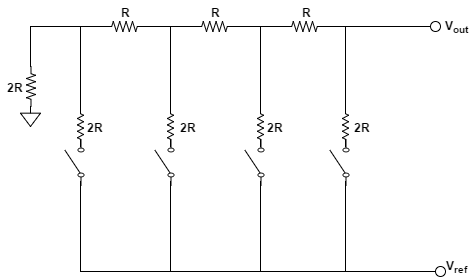
\includegraphics[scale=0.8]{SA-ADC.png}
\centering
\caption{Block diagram of a 4-bit Successive-Approximation ADC}
\end{figure}
\end{itemize}

\section{Mixed Circuit based PUF}


\section{Evaluation}

\section{Conclusion}
